% !TEX program = lualatex
\documentclass[a4paper,10pt,oneside,openany]{ltjsreport}
\usepackage[margin=21mm,top=19mm,bottom=20mm]{geometry}
\usepackage[haranoaji]{luatexja-preset}
\usepackage{amsmath,amssymb,graphicx,booktabs,longtable,xcolor,float}
\usepackage[unicode,colorlinks=true,linkcolor=blue!45!black,urlcolor=blue!45!black]{hyperref}
\usepackage{caption}
\captionsetup{font=small,labelfont=bf}
\setcounter{tocdepth}{0}
\setlength{\parskip}{0.45em}
\setlength{\parindent}{1em}
\raggedbottom
\newcommand{\sourcefile}[1]{{\small\texttt{\detokenize{#1}}}}
\begin{document}


\title{\Huge 実験3\\[0.6em]\LARGE 粒子数依存性\\[1em]\large 一次元HubbardモデルのUHF計算}

\author{保存結果の解析レポート}\date{2026年11月2日}\maketitle

\chapter*{概要}

$U=4$、スピン非偏極のまま $N_e=46,48,50,52,54$ と変えた。10ケース中、収束したのは半充填の2ケースと $N_e=48$ のPBCだけである。粒子数を半充填からずらすと電荷・磁化に局所的な変調が生じ、今回の反復法では収束が著しく遅くなる。未収束の最終値は傾向を調べる暫定値として扱う。

対象は10ケース、保存図41枚である。収束は3ケース、未収束は7ケース。本書では生成物の種類ごとに章を設け、同じ条件のOBCとPBCを並べて読む。

\tableofcontents

\chapter{計算ログ：条件と最終結果}

\sourcefile{uhf_results.txt}

\section*{計算条件と量の定義}

$L=50$、$t=1$、温度 $T=0$、外部電場なし。全エネルギーと軌道エネルギーは $t$ を単位とする。
OBCは開放端、PBCはサイト50と1も接続する周期境界である。$N_e=N_\uparrow+N_\downarrow$、$\Delta N=N_\uparrow-N_\downarrow$ と定義する。
収束判定は混合前の密度残差 $r<10^{-10}$、最大反復回数は10000である。
表の「未」は未収束の最終再評価値であり、その桁数は精度保証ではない。

\begin{center}\small\setlength{\tabcolsep}{4pt}
\begin{longtable}{lrrrr}
\toprule
条件 & $N_e$ & $\Delta N$ & $U/t$ & mixing \\ \midrule
\endhead
Ne46 & 46 & 0 & 4 & 0.25 \\
Ne48 & 48 & 0 & 4 & 0.25 \\
Ne50 & 50 & 0 & 4 & 0.25 \\
Ne52 & 52 & 0 & 4 & 0.25 \\
Ne54 & 54 & 0 & 4 & 0.25 \\
\bottomrule\end{longtable}\end{center}

\section*{最終エネルギー}

$E=E_{\rm kin}+E_{\rm int}$、$E_{\rm int}=U\sum_i n_{i\uparrow}n_{i\downarrow}$。全エネルギーは占有軌道固有値の単純な総和ではなく、平均場の二重計数を除いた量である。

\begin{center}\small\setlength{\tabcolsep}{4pt}
\begin{longtable}{lrrrr}
\toprule
条件/境界 & 状態 & $E$ & $E_{\rm kin}$ & $E_{\rm int}$ \\ \midrule
\endhead
Ne46/OBC & 未 & -26.320110741 & -46.133212224 & 19.813101482 \\
Ne46/PBC & 未 & -26.763038523 & -46.912200597 & 20.149162074 \\
Ne48/OBC & 未 & -24.666586286 & -44.621264272 & 19.954677986 \\
Ne48/PBC & 収束 & -24.747304988 & -44.512677377 & 19.765372388 \\
Ne50/OBC & 収束 & -23.013070704 & -43.110712440 & 20.097641737 \\
Ne50/PBC & 収束 & -23.455261995 & -43.889991764 & 20.434729770 \\
Ne52/OBC & 未 & -16.666586286 & -44.621264272 & 27.954677986 \\
Ne52/PBC & 未 & -17.108777629 & -45.400568850 & 28.291791221 \\
Ne54/OBC & 未 & -10.320110741 & -46.133212224 & 35.813101482 \\
Ne54/PBC & 未 & -10.763038939 & -46.912219496 & 36.149180557 \\
\bottomrule\end{longtable}\end{center}

$U=4$、スピン非偏極のまま $N_e=46,48,50,52,54$ と変えた。10ケース中、収束したのは半充填の2ケースと $N_e=48$ のPBCだけである。粒子数を半充填からずらすと電荷・磁化に局所的な変調が生じ、今回の反復法では収束が著しく遅くなる。未収束の最終値は傾向を調べる暫定値として扱う。

\section*{原資料と再利用}

出典は \sourcefile{results_vault/experiment_03/} 内の各条件/OBC・PBCのログ、CSV、PNG。\\ 補助資料は \sourcefile{experiment_conditions.md} と \sourcefile{uhf.jl}。値は保存済みの結果から採り、SCFを再実行していない。

条件名は原資料のディレクトリ名である。Ne50は実験2の再利用。

再利用データは独立した追加試行ではない。本書の解釈は保存された有限サイズ・UHF解の範囲に限る。

\chapter{密度CSV：電荷分布と二重占有}

\sourcefile{density_checkpoint.csv}

CSVの50サイトすべてから $q_i=n_{i\uparrow}+n_{i\downarrow}$、$m_i=n_{i\uparrow}-n_{i\downarrow}$、
$D=L^{-1}\sum_i n_{i\uparrow}n_{i\downarrow}$ を計算した。密度の各スピン成分は0以上1以下で、総和は指定した粒子数に一致することを確認した。未収束時のCSVは最後の混合密度を対角化して得た出力密度であり、固定点の密度とは限らない。

\begin{center}\small\setlength{\tabcolsep}{4pt}
\begin{longtable}{lrrrr}
\toprule
条件/境界 & 状態 & $\min q_i$ & $\max q_i$ & $D$ \\ \midrule
\endhead
Ne46/OBC & 未 & 0.673299 & 0.999979 & 0.099066 \\
Ne46/PBC & 未 & 0.695545 & 0.999832 & 0.100746 \\
Ne48/OBC & 未 & 0.679888 & 1.000000 & 0.099773 \\
Ne48/PBC & 収束 & 0.589351 & 0.999999 & 0.098827 \\
Ne50/OBC & 収束 & 1.000000 & 1.000000 & 0.100488 \\
Ne50/PBC & 収束 & 1.000000 & 1.000000 & 0.102174 \\
Ne52/OBC & 未 & 1.000000 & 1.320112 & 0.139773 \\
Ne52/PBC & 未 & 1.000000 & 1.321044 & 0.141459 \\
Ne54/OBC & 未 & 1.000021 & 1.326701 & 0.179066 \\
Ne54/PBC & 未 & 1.000168 & 1.304226 & 0.180746 \\
\bottomrule\end{longtable}\end{center}

OBCの電荷密度範囲は $N_e=46$ で約0.6733--1.0000、$N_e=48$ で約0.6799--1.0000となり、ホールが均一に広がった状態ではない。電子を加えた52、54では対応して1以上の密度が現れる。OBCでは46と54、48と52で磁化の平均絶対値がそれぞれ一致するが、いずれも未収束同士の比較である。

\chapter{SCFエネルギー：反復による変化}

\sourcefile{scf_energy.png}

OBCの最終記録では $E(52)-E(48)=8$、$E(54)-E(46)=16$ で、運動エネルギーは対応する組で一致する。この差は二部格子上の粒子・正孔変換に対応する $U(N_e-L)$ のエネルギーずれと整合する。ただしPBCの48と52は別の解・反復段階にあり、その対応が同じようには成立していない。粒子数が異なる系の全エネルギーをそのまま比較して、どちらの充填が安定かとは結論できない。

各図の横軸は反復回数、縦軸は各反復で評価した全エネルギーである。図ごとに軸範囲が異なるため、見かけの傾きだけを比較しない。最終ログ値は反復終了後の再評価であり、履歴の最終点とわずかに異なる場合がある。

\begin{center}\small\setlength{\tabcolsep}{4pt}
\begin{longtable}{lrrr}
\toprule
条件/境界 & 初回 $E$ & 最終 $E$ & 最後の履歴の $|\Delta E|$ \\ \midrule
\endhead
Ne46/OBC & -21.940669 & -26.320111 & $8.439\times10^{-9}$ \\
Ne46/PBC & -22.628191 & -26.763039 & $1.436\times10^{-9}$ \\
Ne48/OBC & -19.559056 & -24.666586 & $8.800\times10^{-11}$ \\
Ne48/PBC & -20.167507 & -24.747305 & $0$ \\
Ne50/OBC & -17.140038 & -23.013071 & $0$ \\
Ne50/PBC & -17.699645 & -23.455262 & $0$ \\
Ne52/OBC & -11.559056 & -16.666586 & $8.800\times10^{-11}$ \\
Ne52/PBC & -12.167631 & -17.108778 & $9.400\times10^{-11}$ \\
Ne54/OBC & -5.940669 & -10.320111 & $8.439\times10^{-9}$ \\
Ne54/PBC & -6.628191 & -10.763039 & $8.100\times10^{-10}$ \\
\bottomrule\end{longtable}\end{center}

\begin{figure}[H]\centering

\begin{minipage}{0.49\linewidth}\centering

\textbf{OBC：未収束・暫定}\par

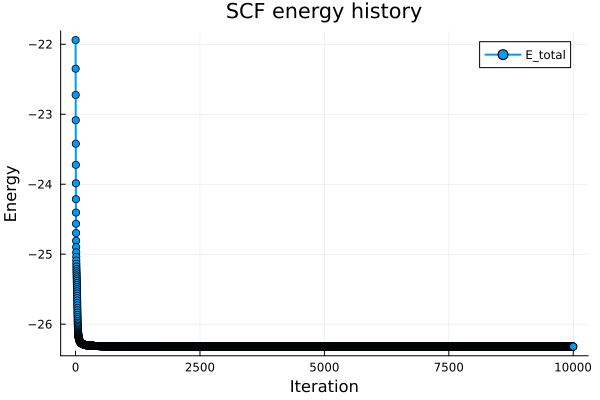
\includegraphics[width=\linewidth]{../../results_vault/experiment_03/Ne46/OBC/scf_energy.png}

\end{minipage}\hfill%
\begin{minipage}{0.49\linewidth}\centering

\textbf{PBC：未収束・暫定}\par

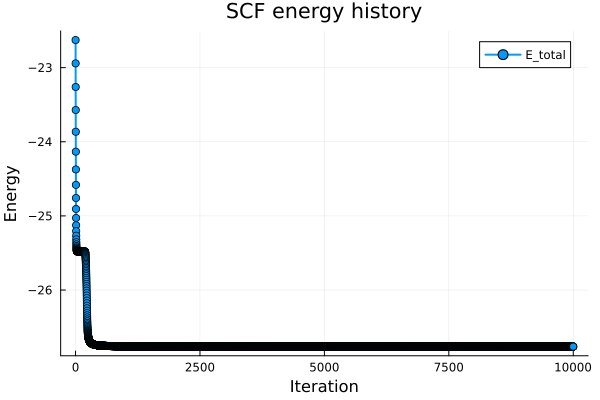
\includegraphics[width=\linewidth]{../../results_vault/experiment_03/Ne46/PBC/scf_energy.png}

\end{minipage}

\caption{Ne46。SCFエネルギーの比較。左：OBC、右：PBC。}\end{figure}

\begin{figure}[H]\centering

\begin{minipage}{0.49\linewidth}\centering

\textbf{OBC：未収束・暫定}\par

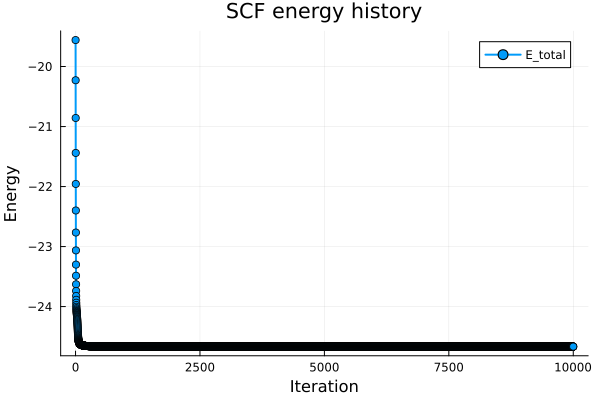
\includegraphics[width=\linewidth]{../../results_vault/experiment_03/Ne48/OBC/scf_energy.png}

\end{minipage}\hfill%
\begin{minipage}{0.49\linewidth}\centering

\textbf{PBC：収束}\par

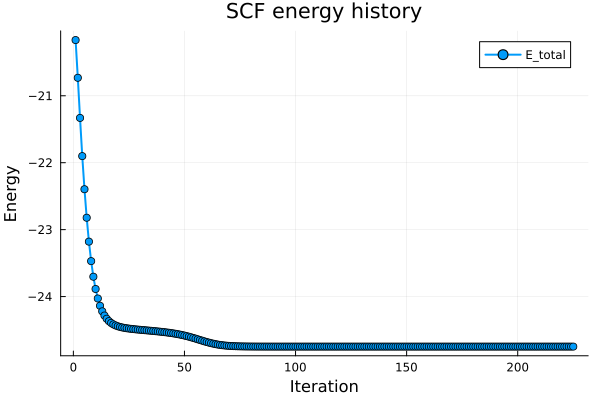
\includegraphics[width=\linewidth]{../../results_vault/experiment_03/Ne48/PBC/scf_energy.png}

\end{minipage}

\caption{Ne48。SCFエネルギーの比較。左：OBC、右：PBC。}\end{figure}

\begin{figure}[H]\centering

\begin{minipage}{0.49\linewidth}\centering

\textbf{OBC：収束}\par

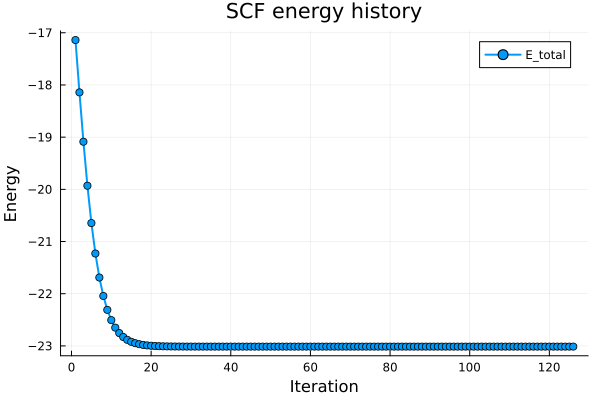
\includegraphics[width=\linewidth]{../../results_vault/experiment_03/Ne50/OBC/scf_energy.png}

\end{minipage}\hfill%
\begin{minipage}{0.49\linewidth}\centering

\textbf{PBC：収束}\par

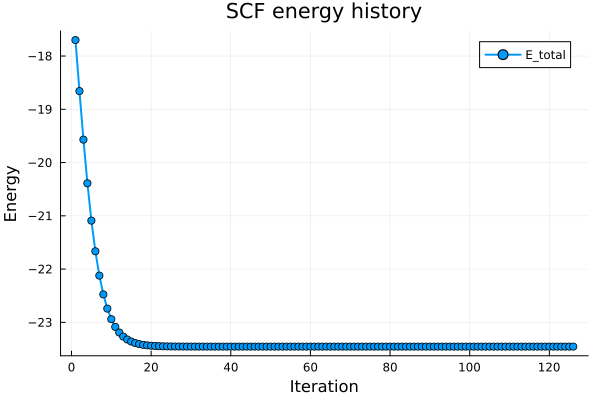
\includegraphics[width=\linewidth]{../../results_vault/experiment_03/Ne50/PBC/scf_energy.png}

\end{minipage}

\caption{Ne50。SCFエネルギーの比較。左：OBC、右：PBC。}\end{figure}

\begin{figure}[H]\centering

\begin{minipage}{0.49\linewidth}\centering

\textbf{OBC：未収束・暫定}\par

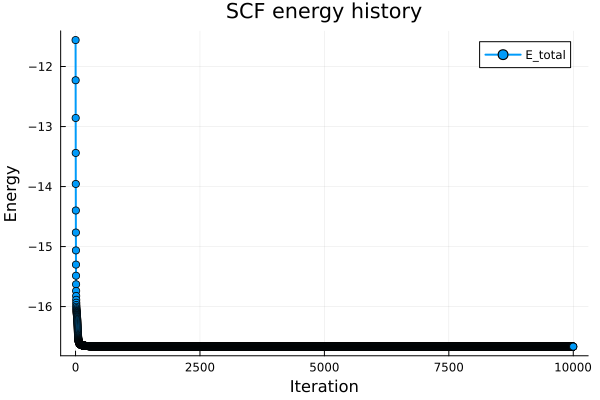
\includegraphics[width=\linewidth]{../../results_vault/experiment_03/Ne52/OBC/scf_energy.png}

\end{minipage}\hfill%
\begin{minipage}{0.49\linewidth}\centering

\textbf{PBC：未収束・暫定}\par

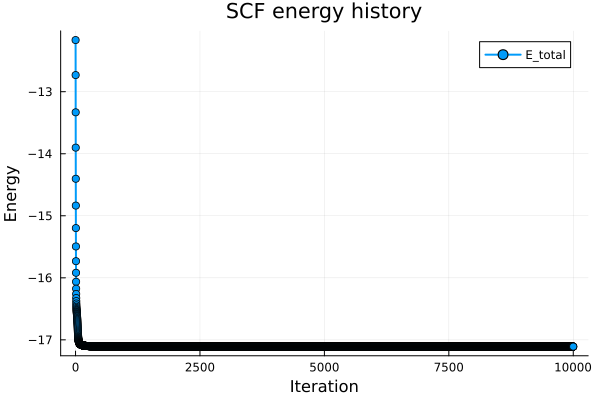
\includegraphics[width=\linewidth]{../../results_vault/experiment_03/Ne52/PBC/scf_energy.png}

\end{minipage}

\caption{Ne52。SCFエネルギーの比較。左：OBC、右：PBC。}\end{figure}

\begin{figure}[H]\centering

\begin{minipage}{0.49\linewidth}\centering

\textbf{OBC：未収束・暫定}\par

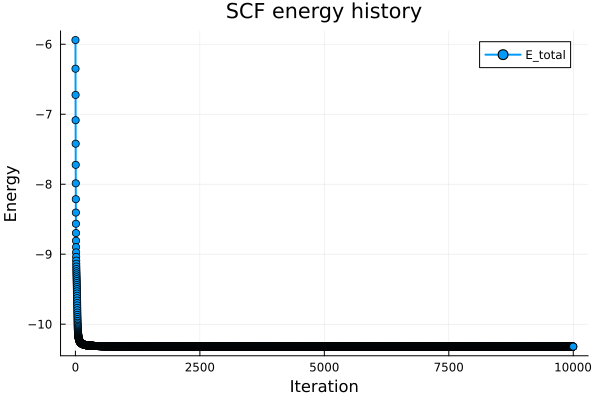
\includegraphics[width=\linewidth]{../../results_vault/experiment_03/Ne54/OBC/scf_energy.png}

\end{minipage}\hfill%
\begin{minipage}{0.49\linewidth}\centering

\textbf{PBC：未収束・暫定}\par

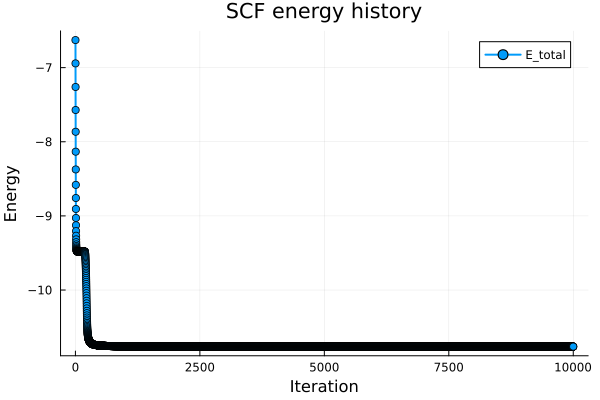
\includegraphics[width=\linewidth]{../../results_vault/experiment_03/Ne54/PBC/scf_energy.png}

\end{minipage}

\caption{Ne54。SCFエネルギーの比較。左：OBC、右：PBC。}\end{figure}

\chapter{SCF残差：自己無撞着性}

\sourcefile{scf_residual.png}

未収束例の残差は $4.026\times10^{-6}$ から $3.778\times10^{-5}$ 程度で、判定値 $10^{-10}$ を大幅に上回る。46および54のOBCでは途中で残差が減少した後に再増加する。エネルギー曲線が平坦でも密度の緩和は完了していない。48のPBCは225反復で収束したが、OBCは10000反復でも未収束で、境界条件による収束経路の違いが顕著である。

残差は $r=\max_{i,\sigma}|F[n]_{i\sigma}-n_{i\sigma}|$。表は最終再評価値である。収束時には出力密度を採用してから再評価するため、履歴図の最後の残差とは同じとは限らない。

\begin{center}\small\setlength{\tabcolsep}{4pt}
\begin{longtable}{lrrr}
\toprule
条件/境界 & 状態 & 反復数 & 最終残差 \\ \midrule
\endhead
Ne46/OBC & 未 & 10000 & $3.778\times10^{-5}$ \\
Ne46/PBC & 未 & 10000 & $1.574\times10^{-5}$ \\
Ne48/OBC & 未 & 10000 & $4.026\times10^{-6}$ \\
Ne48/PBC & 収束 & 225 & $4.944\times10^{-11}$ \\
Ne50/OBC & 収束 & 126 & $3.266\times10^{-11}$ \\
Ne50/PBC & 収束 & 126 & $3.263\times10^{-11}$ \\
Ne52/OBC & 未 & 10000 & $4.026\times10^{-6}$ \\
Ne52/PBC & 未 & 10000 & $4.750\times10^{-6}$ \\
Ne54/OBC & 未 & 10000 & $3.778\times10^{-5}$ \\
Ne54/PBC & 未 & 10000 & $1.191\times10^{-5}$ \\
\bottomrule\end{longtable}\end{center}

\begin{figure}[H]\centering

\begin{minipage}{0.49\linewidth}\centering

\textbf{OBC：未収束・暫定}\par

\includegraphics[width=\linewidth]{../../results_vault/experiment_03/Ne46/OBC/scf_residual.png}

\end{minipage}\hfill%
\begin{minipage}{0.49\linewidth}\centering

\textbf{PBC：未収束・暫定}\par

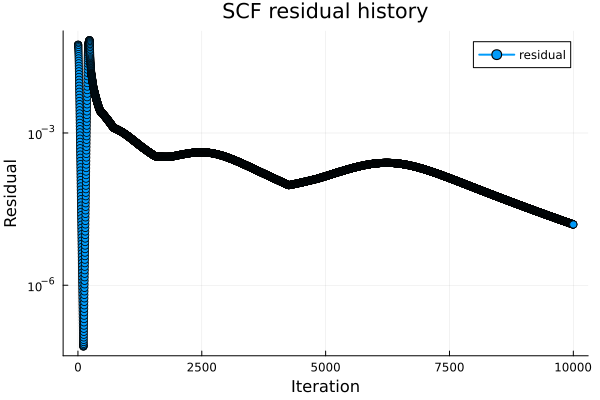
\includegraphics[width=\linewidth]{../../results_vault/experiment_03/Ne46/PBC/scf_residual.png}

\end{minipage}

\caption{Ne46。SCF残差の比較。左：OBC、右：PBC。}\end{figure}

\begin{figure}[H]\centering

\begin{minipage}{0.49\linewidth}\centering

\textbf{OBC：未収束・暫定}\par

\includegraphics[width=\linewidth]{../../results_vault/experiment_03/Ne48/OBC/scf_residual.png}

\end{minipage}\hfill%
\begin{minipage}{0.49\linewidth}\centering

\textbf{PBC：収束}\par

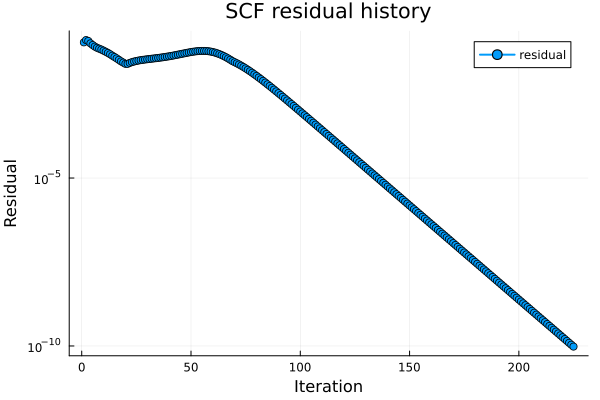
\includegraphics[width=\linewidth]{../../results_vault/experiment_03/Ne48/PBC/scf_residual.png}

\end{minipage}

\caption{Ne48。SCF残差の比較。左：OBC、右：PBC。}\end{figure}

\begin{figure}[H]\centering

\begin{minipage}{0.49\linewidth}\centering

\textbf{OBC：収束}\par

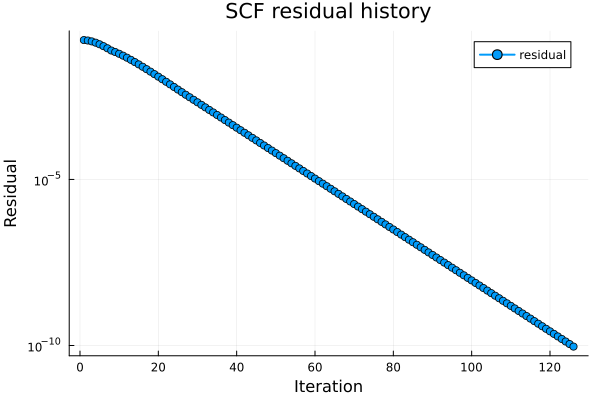
\includegraphics[width=\linewidth]{../../results_vault/experiment_03/Ne50/OBC/scf_residual.png}

\end{minipage}\hfill%
\begin{minipage}{0.49\linewidth}\centering

\textbf{PBC：収束}\par

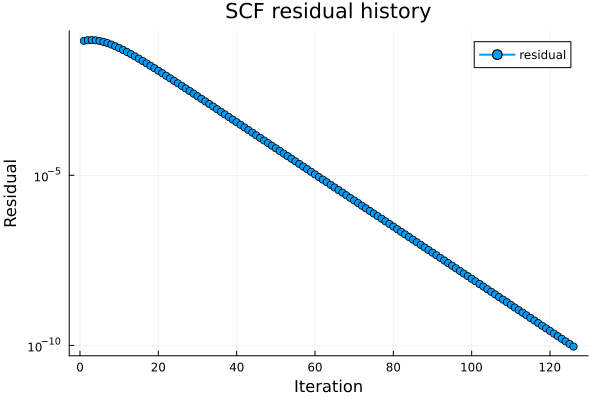
\includegraphics[width=\linewidth]{../../results_vault/experiment_03/Ne50/PBC/scf_residual.png}

\end{minipage}

\caption{Ne50。SCF残差の比較。左：OBC、右：PBC。}\end{figure}

\begin{figure}[H]\centering

\begin{minipage}{0.49\linewidth}\centering

\textbf{OBC：未収束・暫定}\par

\includegraphics[width=\linewidth]{../../results_vault/experiment_03/Ne52/OBC/scf_residual.png}

\end{minipage}\hfill%
\begin{minipage}{0.49\linewidth}\centering

\textbf{PBC：未収束・暫定}\par

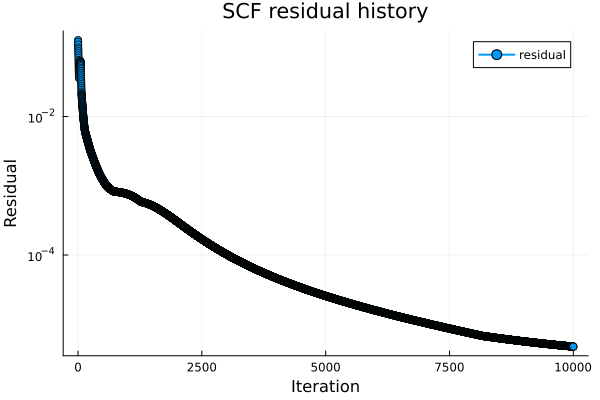
\includegraphics[width=\linewidth]{../../results_vault/experiment_03/Ne52/PBC/scf_residual.png}

\end{minipage}

\caption{Ne52。SCF残差の比較。左：OBC、右：PBC。}\end{figure}

\begin{figure}[H]\centering

\begin{minipage}{0.49\linewidth}\centering

\textbf{OBC：未収束・暫定}\par

\includegraphics[width=\linewidth]{../../results_vault/experiment_03/Ne54/OBC/scf_residual.png}

\end{minipage}\hfill%
\begin{minipage}{0.49\linewidth}\centering

\textbf{PBC：未収束・暫定}\par

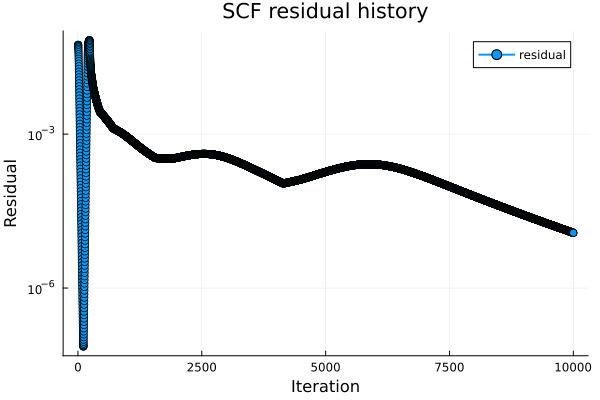
\includegraphics[width=\linewidth]{../../results_vault/experiment_03/Ne54/PBC/scf_residual.png}

\end{minipage}

\caption{Ne54。SCF残差の比較。左：OBC、右：PBC。}\end{figure}

\chapter{軌道エネルギー：準位構造}

\sourcefile{final_orbital_energies.png}

半充填の大きな準位分離に対し、ドープした条件では中央付近に中間的な準位や細かい段差が見える。48のPBCには他の条件と異なる準位構造も見られる。未収束例の固有値は最後の混合密度に対する平均場の値なので、収束した励起スペクトルや金属・絶縁体の確定判定には使わない。

横軸はエネルギー昇順の軌道番号、縦軸は $h_\sigma=h_0+U\operatorname{diag}(n_{\bar\sigma})$ の固有値である。固有値の数値ファイルは保存されていないため、図からの解釈は定性的なものに留める。未収束例をCSVから再対角化すると保存図とは異なる平均場になる可能性があり、本書ではその置換を行わない。

\begin{figure}[H]\centering

\begin{minipage}{0.49\linewidth}\centering

\textbf{OBC：未収束・暫定}\par

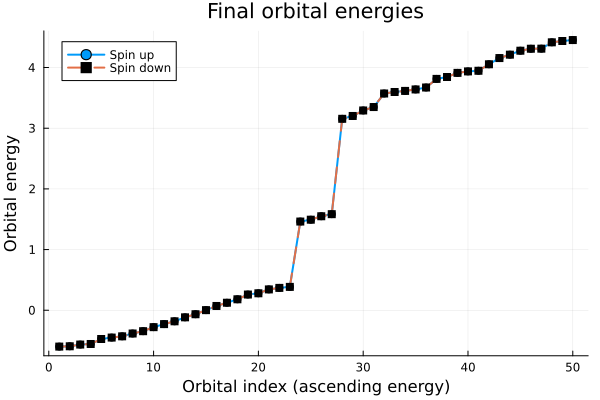
\includegraphics[width=\linewidth]{../../results_vault/experiment_03/Ne46/OBC/final_orbital_energies.png}

\end{minipage}\hfill%
\begin{minipage}{0.49\linewidth}\centering

\textbf{PBC：未収束・暫定}\par

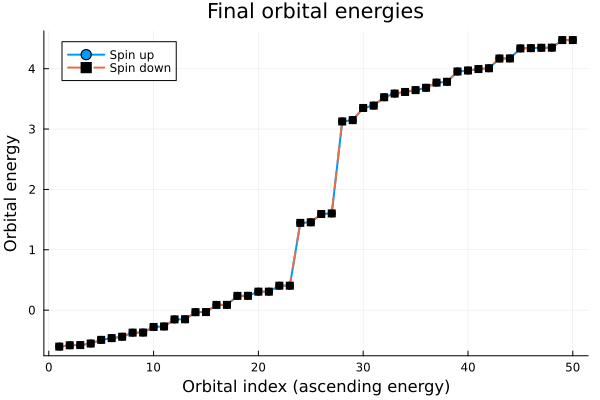
\includegraphics[width=\linewidth]{../../results_vault/experiment_03/Ne46/PBC/final_orbital_energies.png}

\end{minipage}

\caption{Ne46。軌道エネルギーの比較。左：OBC、右：PBC。}\end{figure}

\begin{figure}[H]\centering

\begin{minipage}{0.49\linewidth}\centering

\textbf{OBC：未収束・暫定}\par

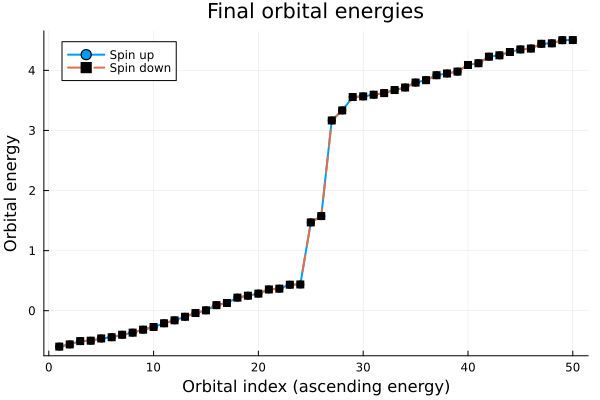
\includegraphics[width=\linewidth]{../../results_vault/experiment_03/Ne48/OBC/final_orbital_energies.png}

\end{minipage}\hfill%
\begin{minipage}{0.49\linewidth}\centering

\textbf{PBC：収束}\par

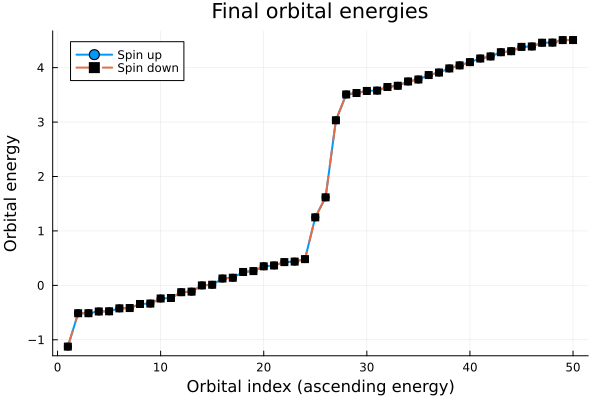
\includegraphics[width=\linewidth]{../../results_vault/experiment_03/Ne48/PBC/final_orbital_energies.png}

\end{minipage}

\caption{Ne48。軌道エネルギーの比較。左：OBC、右：PBC。}\end{figure}

\begin{figure}[H]\centering

\begin{minipage}{0.49\linewidth}\centering

\textbf{OBC：収束}\par

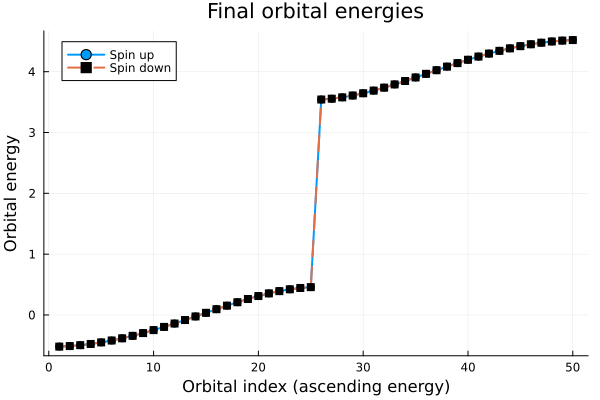
\includegraphics[width=\linewidth]{../../results_vault/experiment_03/Ne50/OBC/final_orbital_energies.png}

\end{minipage}\hfill%
\begin{minipage}{0.49\linewidth}\centering

\textbf{PBC：収束}\par

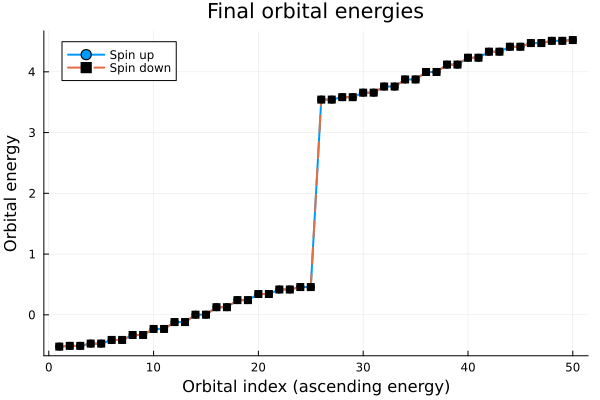
\includegraphics[width=\linewidth]{../../results_vault/experiment_03/Ne50/PBC/final_orbital_energies.png}

\end{minipage}

\caption{Ne50。軌道エネルギーの比較。左：OBC、右：PBC。}\end{figure}

\begin{figure}[H]\centering

\begin{minipage}{0.49\linewidth}\centering

\textbf{OBC：未収束・暫定}\par

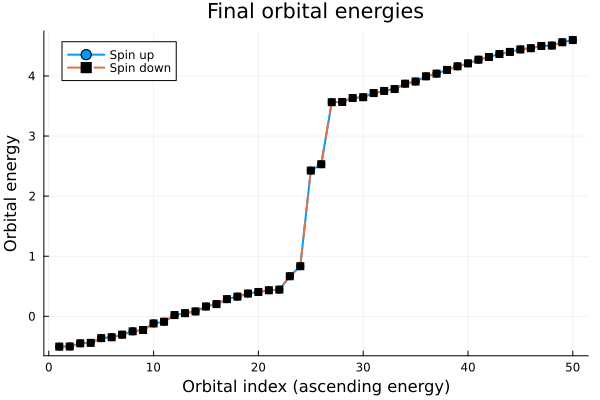
\includegraphics[width=\linewidth]{../../results_vault/experiment_03/Ne52/OBC/final_orbital_energies.png}

\end{minipage}\hfill%
\begin{minipage}{0.49\linewidth}\centering

\textbf{PBC：未収束・暫定}\par

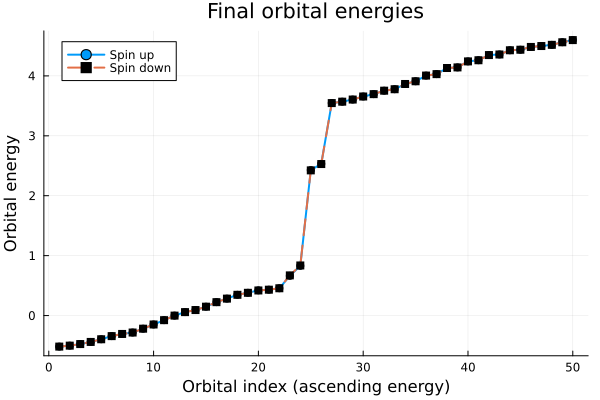
\includegraphics[width=\linewidth]{../../results_vault/experiment_03/Ne52/PBC/final_orbital_energies.png}

\end{minipage}

\caption{Ne52。軌道エネルギーの比較。左：OBC、右：PBC。}\end{figure}

\begin{figure}[H]\centering

\begin{minipage}{0.49\linewidth}\centering

\textbf{OBC：未収束・暫定}\par

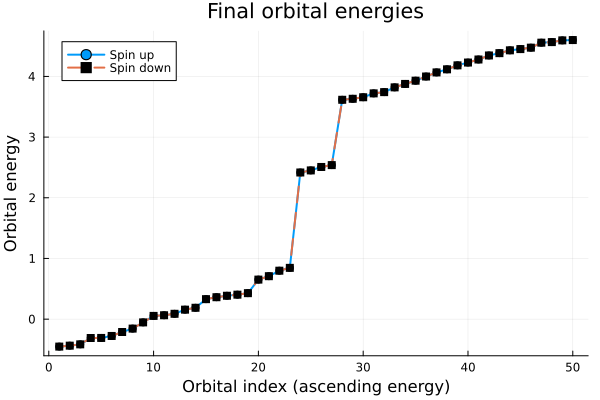
\includegraphics[width=\linewidth]{../../results_vault/experiment_03/Ne54/OBC/final_orbital_energies.png}

\end{minipage}\hfill%
\begin{minipage}{0.49\linewidth}\centering

\textbf{PBC：未収束・暫定}\par

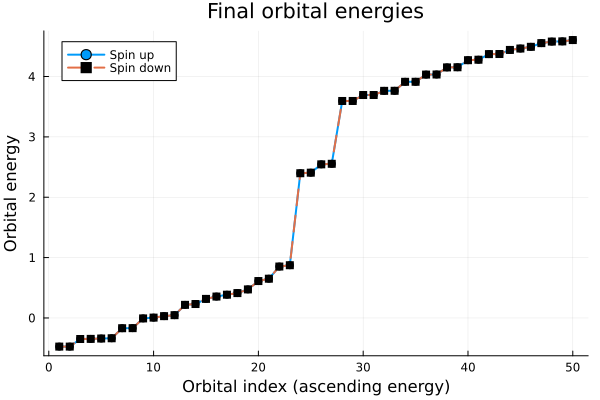
\includegraphics[width=\linewidth]{../../results_vault/experiment_03/Ne54/PBC/final_orbital_energies.png}

\end{minipage}

\caption{Ne54。軌道エネルギーの比較。左：OBC、右：PBC。}\end{figure}

\chapter{局所磁化：空間構造}

\sourcefile{final_magnetization.png}

OBCの $\overline{|m|}$ は半充填の0.773051から48・52で0.711792、46・54で0.649298へ減少する。一方、交互磁化 $M_{\rm AF}$ は0.773051から0.511066、0.244599へより強く低下する。これは局所振幅の減少だけでなく、図に見える符号配列のずれ・磁区構造も寄与するためである。PBCの48の収束解は $\overline{|m|}=0.725832$ で、未収束の52と単純な鏡像関係にない。

$\overline{|m|}=L^{-1}\sum_i|m_i|$、$M_{\rm AF}=|L^{-1}\sum_i(-1)^im_i|$ と定義する。$m_i$ はスピン密度差であり、$\langle S_i^z\rangle=m_i/2$ に対応する。全磁化は $\sum_i m_i=\Delta N$ と粒子数制約で固定される。

\begin{center}\small\setlength{\tabcolsep}{4pt}
\begin{longtable}{lrrr}
\toprule
条件/境界 & 状態 & $\overline{|m|}$ & $M_{\rm AF}$ \\ \midrule
\endhead
Ne46/OBC & 未 & 0.649298 & 0.244599 \\
Ne46/PBC & 未 & 0.649121 & 0.205625 \\
Ne48/OBC & 未 & 0.711792 & 0.511066 \\
Ne48/PBC & 収束 & 0.725832 & 0.690911 \\
Ne50/OBC & 収束 & 0.773051 & 0.773051 \\
Ne50/PBC & 収束 & 0.768964 & 0.768964 \\
Ne52/OBC & 未 & 0.711792 & 0.511066 \\
Ne52/PBC & 未 & 0.707688 & 0.506909 \\
Ne54/OBC & 未 & 0.649298 & 0.244599 \\
Ne54/PBC & 未 & 0.649116 & 0.205498 \\
\bottomrule\end{longtable}\end{center}

\begin{figure}[H]\centering

\begin{minipage}{0.49\linewidth}\centering

\textbf{OBC：未収束・暫定}\par

\includegraphics[width=\linewidth]{../../results_vault/experiment_03/Ne46/OBC/final_magnetization.png}

\end{minipage}\hfill%
\begin{minipage}{0.49\linewidth}\centering

\textbf{PBC：未収束・暫定}\par

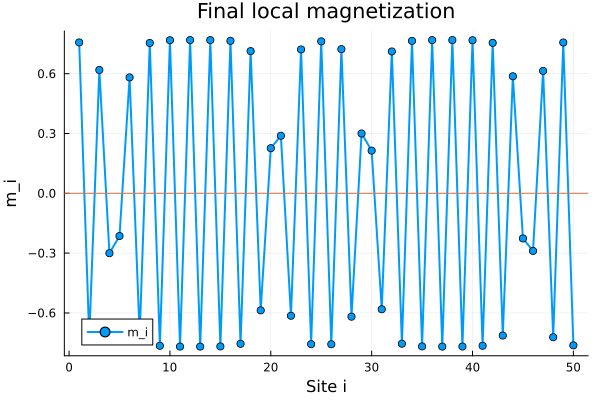
\includegraphics[width=\linewidth]{../../results_vault/experiment_03/Ne46/PBC/final_magnetization.png}

\end{minipage}

\caption{Ne46。局所磁化の比較。左：OBC、右：PBC。}\end{figure}

\begin{figure}[H]\centering

\begin{minipage}{0.49\linewidth}\centering

\textbf{OBC：未収束・暫定}\par

\includegraphics[width=\linewidth]{../../results_vault/experiment_03/Ne48/OBC/final_magnetization.png}

\end{minipage}\hfill%
\begin{minipage}{0.49\linewidth}\centering

\textbf{PBC：収束}\par

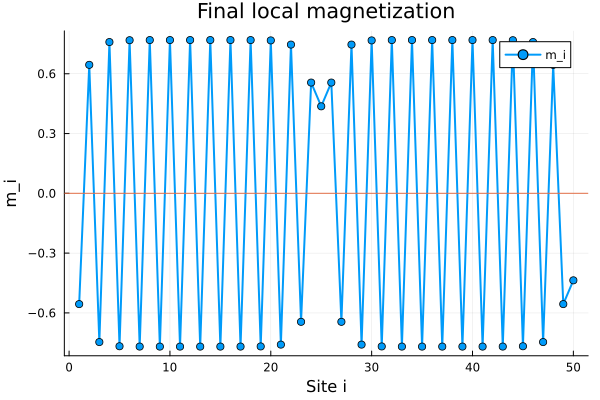
\includegraphics[width=\linewidth]{../../results_vault/experiment_03/Ne48/PBC/final_magnetization.png}

\end{minipage}

\caption{Ne48。局所磁化の比較。左：OBC、右：PBC。}\end{figure}

\begin{figure}[H]\centering

\begin{minipage}{0.49\linewidth}\centering

\textbf{OBC：収束}\par

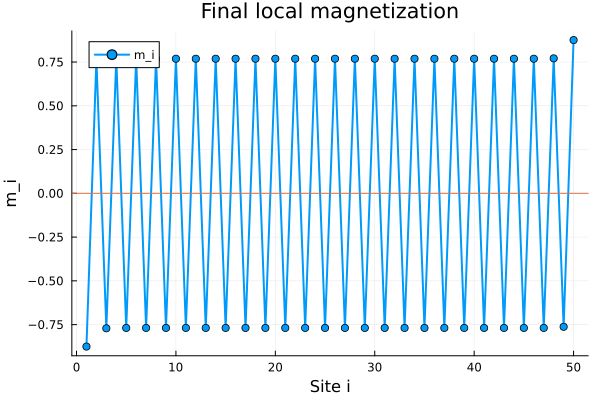
\includegraphics[width=\linewidth]{../../results_vault/experiment_03/Ne50/OBC/final_magnetization.png}

\end{minipage}\hfill%
\begin{minipage}{0.49\linewidth}\centering

\textbf{PBC：収束}\par

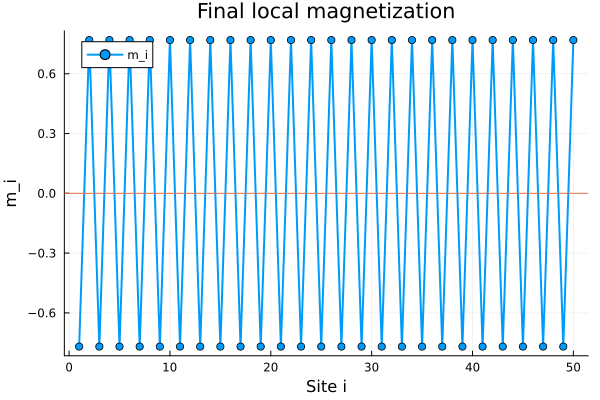
\includegraphics[width=\linewidth]{../../results_vault/experiment_03/Ne50/PBC/final_magnetization.png}

\end{minipage}

\caption{Ne50。局所磁化の比較。左：OBC、右：PBC。}\end{figure}

\begin{figure}[H]\centering

\begin{minipage}{0.49\linewidth}\centering

\textbf{OBC：未収束・暫定}\par

\includegraphics[width=\linewidth]{../../results_vault/experiment_03/Ne52/OBC/final_magnetization.png}

\end{minipage}\hfill%
\begin{minipage}{0.49\linewidth}\centering

\textbf{PBC：未収束・暫定}\par

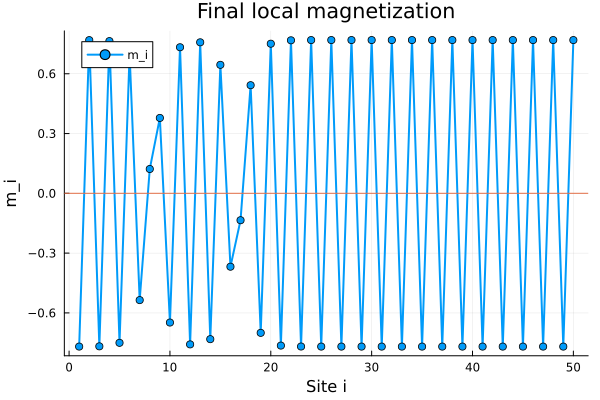
\includegraphics[width=\linewidth]{../../results_vault/experiment_03/Ne52/PBC/final_magnetization.png}

\end{minipage}

\caption{Ne52。局所磁化の比較。左：OBC、右：PBC。}\end{figure}

\begin{figure}[H]\centering

\begin{minipage}{0.49\linewidth}\centering

\textbf{OBC：未収束・暫定}\par

\includegraphics[width=\linewidth]{../../results_vault/experiment_03/Ne54/OBC/final_magnetization.png}

\end{minipage}\hfill%
\begin{minipage}{0.49\linewidth}\centering

\textbf{PBC：未収束・暫定}\par

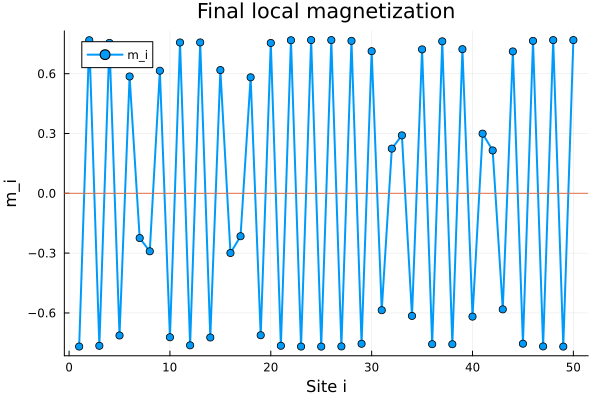
\includegraphics[width=\linewidth]{../../results_vault/experiment_03/Ne54/PBC/final_magnetization.png}

\end{minipage}

\caption{Ne54。局所磁化の比較。左：OBC、右：PBC。}\end{figure}

\chapter{境界条件による全エネルギー差}

\sourcefile{boundary_energy_difference.png}

$\Delta E_{\rm boundary}=E_{\rm PBC}-E_{\rm OBC}$ と定義する。負ならPBC、正ならOBCの保存された解の方が低エネルギーである。両方が収束した組だけを表と図で数値比較し、それ以外をNCとする。

両境界条件が収束しているのは $N_e=50$ のみで、差は $-0.442191290827$ である。他の4条件はNCであり、差が0なのではなく評価を保留している。したがって、この保存結果から境界エネルギー差の粒子数依存曲線を確定することはできない。

\begin{center}\small\setlength{\tabcolsep}{4pt}
\begin{longtable}{lrr}
\toprule
条件 & $\Delta E_{\rm boundary}$ & $\Delta E_{\rm boundary}/L$ \\ \midrule
\endhead
Ne46 & NC & NC \\
Ne48 & NC & NC \\
Ne50 & -0.442191290827 & -0.008843825817 \\
Ne52 & NC & NC \\
Ne54 & NC & NC \\
\bottomrule\end{longtable}\end{center}

\begin{figure}[H]\centering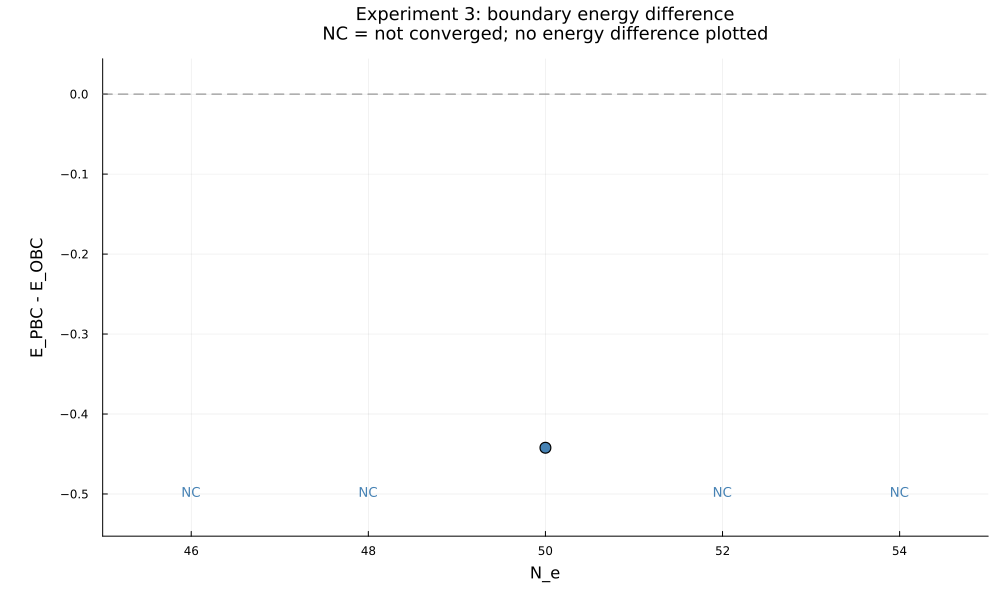
\includegraphics[width=0.9\linewidth]{../../results_vault/experiment_03/boundary_energy_difference.png}\caption{保存済みの境界エネルギー差。NCは未収束の組を示し、差が0であることを意味しない。}\end{figure}

\section*{結論と残された確認}

$U=4$、スピン非偏極のまま $N_e=46,48,50,52,54$ と変えた。10ケース中、収束したのは半充填の2ケースと $N_e=48$ のPBCだけである。粒子数を半充填からずらすと電荷・磁化に局所的な変調が生じ、今回の反復法では収束が著しく遅くなる。未収束の最終値は傾向を調べる暫定値として扱う。

未収束ケースについては残差を満たす解を得た上で、複数の初期密度から同じ状態に到達するかを確認する必要がある。

サイズは50に固定しているため、境界効果と有限サイズ効果の切り分けには別サイズの結果が必要である。

\end{document}